\documentclass[11pt,a4paper]{article}
\usepackage[margin=22mm]{geometry}
\usepackage{fontspec,amsmath,booktabs,graphicx,hyperref,array}
\setmainfont{STIXGeneral}
\setlength{\emergencystretch}{2em}
\begin{document}
\begin{center}{\Large Topic D: written papers and complete programs}\\[4pt]
Human Compression project\end{center}
The three accepted applications recover the declared principal results on
commuting involutions (L066/D1), Suzuki regular polyhedra (L074/D2), and
Hall--Janko geometries (L104/D3). The common paper supplies orbit data,
stabilizer fibers, support counting and panel recognition. The exact
37-row source contract, corrections, retained inputs and exclusions remain
unchanged. This is a comparison of complete extracted manuscript text for
those main results, not equivalence of every printed assertion.

\paragraph{Written papers.}
The three whole source manuscripts cost 47,894 NFC characters without
whitespace. Our whole common paper costs 15,632 and the three whole
applications cost 29,855. Charging the common paper once within Topic D gives
\[
 R_D=\frac{\sum_i c(L_i)}{c(U_D)+\sum_i c(D_i)}
     =\frac{47\,894}{15\,632+29\,855}
     =\frac{47\,894}{45\,487}=\mathbf{1.053}.
\]
The common paper is paid in full even where another topic uses the same idea.

\begin{center}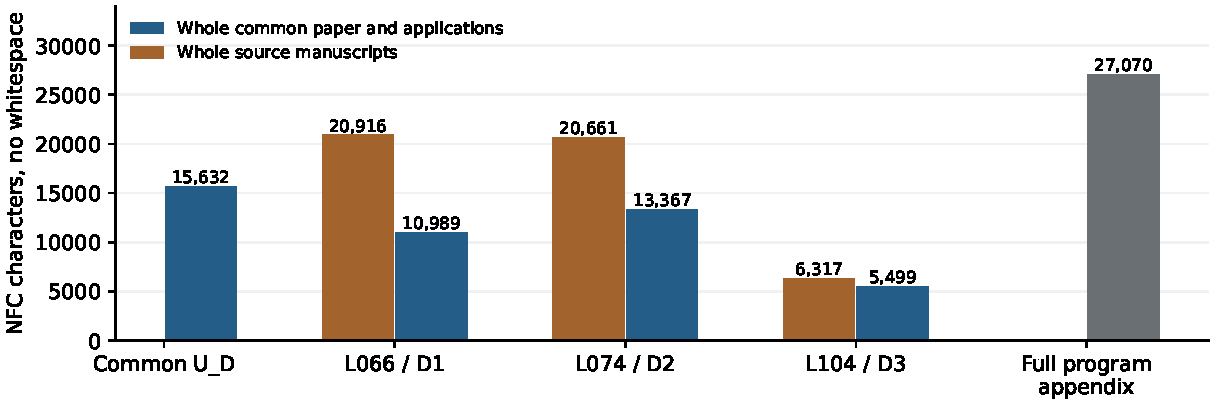
\includegraphics[width=\linewidth]{costs.pdf}\end{center}
\noindent All bars use complete documents after exact running-furniture removal
and occurrence-specific visible-glyph calibration. Unique front matter and
references remain. The grey program bar is a separate comparison below.
These document costs are not a time series or evidence of a sawtooth pattern.

\paragraph{After acquiring the common work.}
After acquiring \emph{the whole common paper and the complete program boundary},
the conditional comparison is $c(L_i)/c(D_i)$. That boundary includes all five
required programs and all three complete diagnostics. Both common theory and
all eight programs are acquired in full before these local comparisons.
\begin{center}\begin{tabular}{lrrr}\toprule
Source / application & Whole source & Whole application & Conditional factor\\\midrule
L066 / D1 & 20,916 & 10,989 & 1.903\\
L074 / D2 & 20,661 & 13,367 & 1.546\\
L104 / D3 & 6,317 & 5,499 & 1.149\\
\bottomrule\end{tabular}\end{center}
These conditional factors do not include the acquisition cost a second time.
The combined written comparison above pays the whole common paper explicitly;
the next comparison also pays every printed program.

\newpage
\paragraph{Including the required program.}
The complete 12-page appendix contains all eight mathematical files: five
required programs and three full diagnostics. It costs 27,070 in the primary
unit, so the separate known-text comparison is
\[
 R_{D,\mathrm{program}}=\frac{47\,894}{45\,487+27\,070}
 =\frac{47\,894}{72\,557}=\mathbf{0.660}.
\]
Here the replacement is longer than the available historical manuscript text.
Historical software and external algorithm construction have unknown cost;
they are not assumed to be free. The comparison states exactly which measured
texts are in its numerator and denominator.

\begin{center}\begin{tabular}{p{.67\linewidth}rr}\toprule
Representation & Denominator & Factor\\\midrule
Written papers & 45,487 & 1.053\\
Written papers plus whole printed appendix & 72,557 & 0.660\\
Written papers plus all eight whole raw programs & 71,672 & 0.668\\\bottomrule
\end{tabular}\end{center}
The whole raw programs cost 26,185, of which 17,209 belongs to the five
required files and 8,976 to the three diagnostics. This is an
\emph{alternative} to the printed appendix, never an additional charge.
Raw metrics are summed file by file, without pruning branches or diagnostic
parts. The two complete execution drivers cost 10,038 separately and are
reported separately from the denominators above. Their 12,765 actual file bytes
are also retained in the machine-readable inventory. One driver retains an
unused historical M22 branch; no M22 result is included.

\paragraph{Sensitivity to the ruler.}
The full tables retain three variants (raw untrimmed, raw selected and
calibrated selected), NFC and NFKC, and five units: 30 coordinates and
180 exact combined/conditional fractions. The middle columns below use
calibrated selected text; the range covers all six variants/normalizations.
\begin{center}\small\begin{tabular}{p{.29\linewidth}rrrr}\toprule
Unit & Written NFC & Written NFKC & Written range & With code NFC\\\midrule
Whitespace tokens & 1.150 & 1.153 & 1.150--1.160 & 0.895\\
Alphanumeric runs & 1.237 & 1.237 & 1.237--1.245 & 0.802\\
Nonspace characters & 1.053 & 1.056 & 1.053--1.064 & 0.660\\
Collapsed characters & 1.069 & 1.072 & 1.069--1.080 & 0.693\\
Collapsed UTF-8 bytes & 1.020 & 1.091 & 1.016--1.099 & 0.680\\
\bottomrule\end{tabular}\end{center}
No one of these units measures intrinsic mathematical difficulty. All use the
same complete-document and program boundary.

\paragraph{Extent and limits.}
The three source PDFs have 9, 12 and 5 physical pages (26 total). Our common
paper has 6 pages, the applications have 5, 6 and 2 (19 scientific pages total),
and the program appendix has 12. All 57 input pages are retained. Vector edges,
formula placement and other unextracted graphical information have unknown
cost. This is an extracted-text coordinate, not a claim to count every visible
mark or all prior research effort. External classical proofs, subgroup catalogue
construction, GAP internals and formal verification costs are separate.

The L104 printed diagrams, full Aut/Cor groups, doubling relation and supplement
annotations are not all recovered; their source text is nevertheless part of
the complete manuscript numerator. The L066 reversal/regularity qualifications
and the retained Suzuki classification remain explicit. The corrected extraction
uses original PDF bytes for fourteen L066 brackets previously confused with
brace pieces. This is an extracted-character/encoding collision, not a
ToUnicode-table collision: that font has no such stream. Only calibrated UTF-8
lengths changed by $-28$; the primary character counts did not change.
Input acceptance and numerical admission are recorded separately. No new
source, conjecture or formal theorem credit follows from this measurement.
\end{document}
